\documentclass[11pt]{article}
\usepackage{parskip}
\usepackage{geometry} \geometry{ letterpaper, total={170mm,257mm}, left=27mm,
right=27mm, top=20mm, bottom=20mm }
\usepackage[dvipsnames]{xcolor}
\usepackage{graphicx} 
%\graphicspath{ {\string~/Desktop/UW/CS\ 246/project/cc3k-dd2/} }
\usepackage{latexsym,amsfonts,amssymb,amsthm,amsmath}
\usepackage{graphpap}
\usepackage{tkz-euclide}
\usepackage{enumitem} 
\setlist[enumerate]{itemsep=0mm}
\usepackage{cases}
\usepackage{hyperref}
\hypersetup{ colorlinks=true, linktoc=all,
linkcolor=black,}
%\usetkzobj{all}
\theoremstyle{plain} \newtheorem{theorem*}{Theorem}[subsection]
\newtheorem{theorem}{Theorem}[subsection]
\newtheorem{thm}{\textit{Theorem}}[subsection]
\newtheorem{definition}{Definition}[subsection]
\newtheorem{algorithm}{Algorithm}[subsection]

\begin{document}

\begin{center}
{\LARGE \textbf{CS 246 Final Project Design}}\\
\vspace{0.15 in}
Xinyan Lin, Hanyu Xu, Rivers Chen\\ 
\vspace{0.07 in} August, 2020 
\end{center}

\vspace{0.3 in} 
\section{OVERVIEW} 
The game of ChamberCrawler3000 is a roguelike game in which the player’s goal
is to reach the exit at the top floor of the five-floor map.  

Basic structure:
\begin{center}
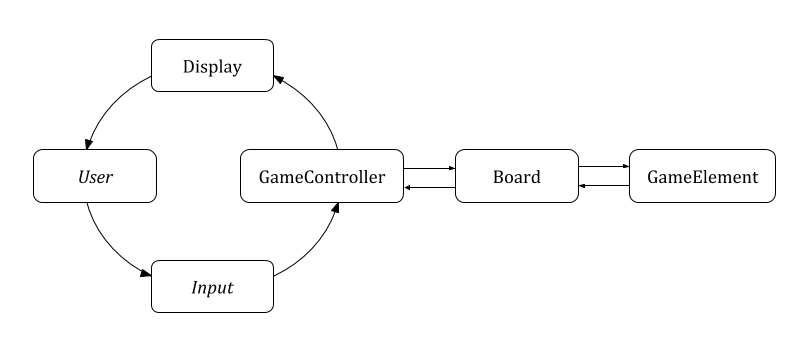
\includegraphics[width=0.7\textwidth]{Flow Chart Cutted.png}
\end{center}

The game follows the OOP design principle, where all actions from clients
should be processed in the \texttt{GameController} class. The 
\texttt{GameController} then does operations on \texttt{Board} or calls 
of functions of \texttt{Board} to change the state of \textsf{floor} of
\texttt{Board}. \textsf{floor} is a 3d vector that shared pointers to
contains all game elements. \texttt{Board} will then access these pointers'
methods to accomplish any tasks required.\\



%------------------------------------------------------------------------------
%------------------------------------------------------------------------------
%-----------------------------------------------------------------------------
%------------------------------------------------------------------------------
%------------------------------------------------------------------------------
%------------------------------------------------------------------------------
\section{DESIGN} 

\subsection{System Components}
%\begin{description} \item 

\subsubsection{Game Element}

All objects are inherited under an abstract class \texttt{GameElement}. which
has game element's x and y positions and their char to display as attributes.
\texttt{GameElement} has three direct subclasses \texttt{Living} and
\texttt{NonLiving}, and \texttt{Architect}.


\subsubsection{Living Characters}

The \texttt{Living} class is an abstract superclass for
\texttt{PlayerCharacter} and \texttt{EnemyCharacter}.  \texttt{Living} contains
character's race, HP, Def, Atk as attributes, and provides their corresponding
accessors and mutators.

%The \texttt{PlayerCharacter} class and \texttt{EnemyCharacter} class are
%features like hp, atk, def, and the ability to attack others, the common
%behaviours of \texttt{PlayerCharacter} and \texttt{EnemyCharacter} are put in
%the base class Living.  Then, both PlayerCharacter and EnemyCharacter inherit
%from the Living class, but also have extra features different from the base
%class.
Under \texttt{PlayerCharacter} and \texttt{EnemyCharacter}, each distinct race
is implemented as a subclass of them.  For player characters, the different
basic stats (hp, atk, def) of different races are initialized with default
value in the constructor of each race respectively.  For the special ability of
different races, the template method design pattern is applied. For example,
shade has its score magnified by 1.5. This is achieved by overriding the score
accessor of \texttt{PlayerCharacter} in the \texttt{Shade} class and return 1.5
* score instead of actual score. For another example, goblin gains 5 gold for
every slained enemy. This is achieved by overriding the \textsf{slain} function
of \texttt{PlayerCharacter} in the \texttt{Goblin} class.  Beside the normal
function flow, 5 extra gold is added to the score of the goblin.  Using the
template method allows each race to override and modify certain steps to
implement their special abilities, but also reuses code for common features.
The implementation of different enemy character races is similar to player
characters, which also applies template method.

\subsubsection{NonLiving Items}

Both \texttt{Potion} and \texttt{Treasure} inherit the \texttt{NonLiving}
superclass which inherits from \texttt{GameElement}.

The \texttt{Potion} classes use the decorator design pattern.  The potions
player character drinks exist as decorators to the player character’s status,
and PC holds a pointer to a concrete component class of “no effect” potion
initially.  This way potions can be easily added and removed when needed, and
their effects can be calculated independent of player character. Since potions
affecting attack and defense are only effective in the current floor, they are
removed when the PC reaches the next floor.  

The \texttt{Treasure} class uses a similar design as the potion class. For each
of the gold size, a specific enum class type exists in the header file which
integer value corresponds to its size. When constructing a treasure, the client
does not need to know necessarily the actual size of the treasure type. Unlike
\texttt{Potion} class, the player character is responsible for adding the value
of the treasure to its score field. A special case is for \texttt{DragonHoard},
since it can only be picked up after the dragon guarding it is slain, a
dragon hoard will return 0 from its \textsf{getAmount} method, 
indicating that it cannot be picked up yet.  


\subsubsection{Architecture}

The \texttt{Architect} class, for Architectures, is a direct subclass 
of \texttt{GameElement}. It is used for floor tiles, walls, passages, doorways,
and also empty spaces. Except the three attributes inherited from
\texttt{GameElement}, \texttt{Architect}
also contains \textsf{chamberInd} as an attribute.
The \textsf{chamberInd} for each floor tiles (`\ .\,') is initialized to
the index of chamber it is in, and other architectures it's just the default
value $0$.
%\texttt{Architect}s will fill the first positions of 1-dimensional
%vectors in the \textsf{floor} of \texttt{Board}. 


\subsubsection{Board}

The \texttt{Board} class stores all gameElements as shared pointers. 
It contains a 3d vector \textsf{floor}, which each 
\textsf{floor[i][j]} represents a square on the board, and is implemented as an
1-dimensional vector of game element shared pointers. The first position is
always an \texttt{Architect} object, 
and any other game elements ``standing" on this
position is pushed back onto this 1-dimensional vector.

\texttt{Board} also contains vector of shared pointer of 
\texttt{EnemyCharacter} named \textsf{enemyList} which is renewed at each level.
This vector has all enemies on current \textsf{floor} that moves 
(so dragons will not be in this vector).
When we move enemies at the end of each round, each enemy in the vector 
that are not beside pc will
be removed from \textsf{floor} in order then randonly assign a new position.
After that, this \textsf{enemyList} will be sorted according to new position.



\subsubsection{GameController}

The \texttt{GameController} acts as a controller of the whole game,
it is a friend class of \texttt{Board}. 
The functions in \texttt{GameController} will access
the game elements on \textsf{floor} to handle tasks such as setup of
\textsf{floor}, spawn of PC and enemies, move PC and enemies, etc.  The
specific design of how these are complished will be in section 2.2.3.

\texttt{GameController} holds a shared pointer to our player character and also
holds attributes of x and y position of the stair of current floor.

\subsubsection{Display} 

By design, everything relating to output of the game
components should be handled by \texttt{display}. \texttt{display} defines a
set of flags corresponding to various possible states of the game. Only one
display object exists in the program as a global variable, so that any other
objects can pass one of the flags to \texttt{display} when needed.  In
addition, to increase flexibility, \texttt{display} can accept a string
directly and append/prepend it to the game message.\\





\subsection{Features}

\subsubsection{Setup}
The setup of each floor involves the following steps:
\begin{enumerate}[leftmargin=*]%[noitemsep]
\item If at initial level, player select race of pc, 
	use a character to store this race.
\item Reset all game elements on \textsf{floor}, then reset \textsf{enmeyList}.
\item 
If no command line argument is provided, 
\begin{enumerate}[leftmargin=*, noitemsep, label=(\roman*)]
\item 
a default floor layout of floor which
only contains architectures will be used to build to fstream.
\item
\texttt{gameController} will use this fstream to setup an empty board, with
only has \texttt{Architect}s. Floor tiles have the index of the chamber they 
are in as \textsf{chamberInd}, all other architectures have 0 as 
\textsf{chamberInd}. 
\item
Use the char player provided to spawn our player character, 
use while loop and \textbf{<srand>} to find a floor tile(`\ .\ '), 
and store the \textsf{chamberInd} of this tile to 
the attribute \textsf{pcChamberInd}. The \textsf{pc} attribute of 
\texttt{gameController} will be set to this player character generated.
\item
\texttt{gameController} will call \textsf{setGameElement}, which calls first
function \textsf{spawnStair}. This function will use while loop to randomly
find a floor tile with different \textsf{chamberInd} from \textsf{pcChamberInd},
and store the x, y coordinates of stair spawned to \textsf{stairX} and 
\textsf{stairY}.
Second, \texttt{Board}'s \textsf{spawnPotion} will be called, which
uses \textbf{srand} to randomly spawn potions around the chamber.
Third, \texttt{Board} \textsf{spawnGold} will be called, when
\texttt{DragonHoard} is spawned, a \texttt{Dragon} is also spawned beside it.
Fourth, \textsf{spawnEnemy} will be called. A chamber and a position inside the
chamber will be randomly generated, and the race of enemy will be randomly
chosen using an int prob, then \textsf{spawnEnmey} will pass this int "prob"
and the position to \textsf{spawnOneEnemy} to make instance of enemy and 
put it on \textsf{floor}, and also pushed back onto \textsf{enemyList}.

\end{enumerate}

If a single command line argument which is the name of a file that specifies
the layout of each of the 5 floors is provided, then, \textsf{readFloor} of
\texttt{gameController} will be called to change each char in the file to an
object on our board. 
Pushing enemies(except dragon) generated to \textsf{enemyList}, and 
use player character spawned to be \textsf{pc} of \texttt{gameController}.

\end{enumerate}



\subsubsection{ Beginning of one round }

At the beginning of each round, the player input a char to indicate the 
action they want to take. 

If that input is used to do game settings. For example, if to reset the game,
the \texttt{gameController} will reset floor level to and break the inner
loop. If the input is to quit the game, then \textsf{displayLose()} of
\texttt{gameController} will be called and game is quit.

Or the player may play the game by move pc(which may include pick of gold),
attack enemy or drink potion, which is discussed below.


\subsubsection{Middle of one round}

The following actions are possible: 
\begin{enumerate}[leftmargin=*]
\item 
\textbf{Move:} 
Check the direction is unoccupied, then revert where it was on
board \textsf{floor} to a floor tile, and push back pc on its new position on
\textsf{floor}. If that direction has a gold of type not dragon hoard, then
pick gold and move to that position. If that direction is a dragon hoard, then
check if dragon is dead, pick gold and move to that position. Then the 
coordinate of \textsf{pc} will be reset to new position.

\item
\textbf{Combat:} 
Combat system between player character and enemy character uses all
observer, visitor and template method. 
\begin{enumerate}[leftmargin=*, noitemsep, label=(\roman*)]
\item
When \textsf{pc} gets within 1 block radius to an enemy, observer pattern
is used to notify the enemy so that the enemy will attack the player character.
\item
Since the damage dealt by an enemy varies based both the race of the enemy and
the player character, visitor pattern and double dispatch are used to implement
an attack. Whenever a character A is trying to attack a character B, it calls
the function \textsf{A.attack(B)}, then \textsf{A.attack(B)} calls \textsf{B.attackedBy(A)}, which is an
equivalent visit function that behaves differently based on the concrete class
type of A (races of A in this case). Such design pattern makes the combat
system clear and straight forward. For different races, damage will be
calculated differently. 
\item 
Furthermore, some races have special interaction
between each other. And template method is applied to handle these interactions.
If pc dies during combat, lose message will be displayed and player will be
asked if they want to start again. 
\item
If enemy is dead, it will be removed from
\textsf{enemyList} and \textsf{floor}. If the enmey is \texttt{Merchant}, 
a \texttt{MerchantHoard} will be put on the position of this Merchant.
If the enemy is \texttt{Human}, a \texttt{Treasure} of type \texttt{NORMAL\_PILE}
will be put on the position of this Merchant, and another 
same type treasure will be put in a random position in the same chamber.
\end{enumerate}

\item
\textbf{Use Potion:}
again, \texttt{gameController} will check there is a potion
at the direction inputted. Then, it will call \textsf{pc}'s
\textsf{drink(std::shared\_ptr<Potion>)} to attach potions to \textsf{pc} as 
decorators. How potions work has been discussed in section 2.1.3. The potion
will then be removed from its position. 
\end{enumerate}

\subsubsection{End of one Round}

After these actions are completed, \textsf{MoveEnemy} will be called,
then \texttt{gameController} will use \textsf{enmeyList} in \texttt{Board}
to move enemy as described in section 2.1.5. Also, \texttt{gameController}
will call \textsf{flushDisplay()} to display. Message displayed include
the \texttt{floor}, stats of current \textsf{pc}, and the action taken.\\

\subsubsection{End of Game}

If player choose to quit the game using 'q', then the game is immediately 
closed with no message displayed.

If during any round, the HP of \textsf{pc} reach 0, we will check this
in \textsf{FlushDisplay}, if HP is 0, \textsf{displayLose} will display
losing message, the player may choose the restart or quit the game.

If \textsf{pc} reach the stair of last floor, that is, the coordinates of
\textsf{pc} are the same as \textsf{stairX} and \textsf{stairY} and 
\textsf{level} equal to 5, then the game wins with winning message displayed,
and \texttt{ScoreBoard} will be displayed (\texttt{ScoreBoard} discussed in
Section 5.3)

\subsubsection{General Structure}
In general, \texttt{GameController}, \texttt{Board} and \texttt{Display} 
follows the Model-View-Controller Architecture (see flow chart in overview). 
\texttt{GameController} acts as the controller, \texttt{Board} acts as the model, 
and \texttt{Display} acts as the view.\\\\










%------------------------------------------------------------------------------
%------------------------------------------------------------------------------
%------------------------------------------------------------------------------
%------------------------------------------------------------------------------
%------------------------------------------------------------------------------
%------------------------------------------------------------------------------
\section{RESILIENCE TO CHANGE}
\subsection{Adding player and enemy characters}
The \texttt{Living} class involves player characters and enemy characters. 
It is designed to follow high cohesion and low coupling. 
In the \texttt{Living} class, each distinct race has its own header and 
implementation files. Thus, a header and an
implementation serves on a single purpose of implementing the specific race. It
demonstrates the high cohesion in our code. The communication between player
character and enemy character happens in combat only. In a combat, function
calls only takes others in as basic parameters without knowing the actual
implementation. It demonstrates the low coupling in our code as different
modules has very low dependencies between each other. 

\subsection{Adding potions}
Since the potion subclasses use the decorator design pattern, which allows us
to easily add new types of potions to the game, as well as designing more
complicated types of potions, such as ones that have dynamic effects depending
on the progress of the game. Its functionality is also independent from the
player character, which is easier to make changes to the potion classes only. 

\subsection{Adding treasures}
The treasure class uses a enum type to define the various size of gold, if
other sizes of gold are need, or if the current size of gold has to be changed,
one simply has to define additional members or modify existing ones in the enum
type and pass the type into the constructor of treasure. The existing code of
generating treasures may not need change at all. If other types of treasure are
need, subclasses of Treasure can be added to accommodate the change. How
treasures are picked up by Player character is defined on the PC’s side, who is
a friend of treasure class, thus no other changes are needed. 

\subsection{Changes to display}
The \texttt{Display} class handles all the standard message the game has by 
having a set
of flags corresponding to various possible states of the game. It also
dynamically read in the game board when printing its content, and thus there is
no need to change the code of display if other player characters and/or enemies
are added to the board.  

\subsection{Add cures library}
If the one would use the curses library in additional to the current input format, 
only a new file for keyboard input interpretation, and a small adjustment to 
game controller. It makes very little change to our current code.

\subsection{Add inventory system}
To add an inventory system ,a new class \texttt{Inventory} with a map of pointer 
to potions and its amount can be added. Then, minor changes are required on potion 
storage, command interpreter, and game controller.

\subsection{Give enemy intelligence}
To give enemy intelligence, detect when PC gets in combat and moves to get out 
of combat. When PC is not in 1 block radius, makes enemy move in the direction 
PC or simply copy PC's movement. It only requires some additional functions in 
\texttt{GameController} and \texttt{EnemyCharacter}.





%------------------------------------------------------------------------------
%------------------------------------------------------------------------------
%------------------------------------------------------------------------------
%------------------------------------------------------------------------------
%------------------------------------------------------------------------------
%------------------------------------------------------------------------------

\vspace{0.3 in}
\section{ANSWERS TO QUESTIONS}

\textbf{Question:}
How could your design your system so that each race could be easily generated?
Additionally, how difficult does such a solution make adding additional races? 

\textbf{Answer:}
The answer for this question is basically the same as answered in due date 1
design. 

As discussed in section 2.1.2, to generate each race easily, 
apply the template method. An abstract superclass \texttt{PlayerCharacter}
(without race) is pure virtual. Then, based on 
the template method, make each race a distinct sub class of 
\texttt{PlayerCharacter} which inherit accessors and mutators from 
\texttt{Living} and \textsf{attack} and \textsf{attackedBy} from 
\texttt{PlayerCharacter}.

Such solution makes adding additional races easily. If an additional race is to
be added, then we would make the race a new sub class inherited from the base
class \texttt{PlayerCharacter}. We would create a header file and a separate 
implementation file for the race. We can override any method required in the 
sub class. Doing so results in high cohesion and low coupling. The new header 
and implementation file serves solely for the purpose of creating a new race.
Also, such implementation will not affect the base class or any other races.\\

\textbf{Question:}
How does your system handle generating different enemies? Is it different from
how you generate the player character? Why or why not? 

\textbf{Answer:}
For how our system handle generating different enemies, the answer is same as
answered in due date 1 design. 

Like for player characters, use template method to generate different enemies,
\texttt{EnemyCharacter} is the abstract base class which will
never tbe initialized, \texttt{EnemyCharacter} will also contain methods called
\textsf{attack} and \textsf{attackedBy}. 
\textsf{attack} is a method called upon the enemy attacking a PC whereas
\textsf{attackedBy} is a method called upon the enemy being attacked by a PC. 
Based on the template method, make each race a 
distinct subclass of \texttt{EnemyCharacter} like we did for player characters,
then these subclasses all inherit accessors and
mutators from \texttt{Living} and \textsf{attack} and \textsf{attackedBy}
from \texttt{EnemyCharacter}.


For the difference between generating player character and enemy character,
our answer is \underline{different} from our due date 1 design. 

As discussed in section 2.2.1, 
\texttt{GameController} has function \textsf{spawnPC} to generate PC with 
required race. For the enemy generation, \texttt{Board} will call its method
\textsf{spawnEnemy}. \textsf{SpawnEnemy} 
has a helper named \textsf{spawnOneEnemy} that can spawn one specified enemy. 
\textsf{SpawnEnemy} randomly generates a chamber and an unoccupied postiion
inside that chamber and then determines an enemy race based on the probability 
distribution, and calls \textsf{spawnOneEnemy} with these information as
parameters to generate each enemy.
It repeats the process 20 times to get 20 random enemies. 

On due date 1, we proposed to use \texttt{Board} class to controll the entire 
game flow. But in actual implementation, we decided to have \texttt{Board} 
and \texttt{GameController} taking different responsibilities of the game flow. 
Doing so increases the cohesion within the classes. We put PC generation in 
\texttt{GameController}, as its generation is related to user inputs. We put 
enemy generation in \texttt{Board}, as it belongs to part of the floor 
initialization and is unrelated to user’s behaviours. Such reason causes the 
generation of player character and enemy character to be different. \\

\textbf{Question:}
How could you implement the various abilities for the enemy characters? Do you
use the same techniques as for the player character races? Explain. 

\textbf{Answer:}
The answer for this question is slightly \underline{different} from the answer 
in due date 1 design. 

The various abilities for the enemy characters will be implemented differently.
In general, they are implemented with visitor pattern, observer pattern, and 
template method.

The implementation of enemy abilities is different from of PC races. PC races
has no special interaction with enemies. Thus, they can be implemented through
changing the information of PC (I.e. fields and methods). But most enemy
abilities have special interaction with PCs (they do damage differently), thus
we use different design patterns and implementations to complete such features. \\


\textbf{Question:}
The Decorator and Strategy patterns are possible candidates to model the
effects of potions, in your opinion, which pattern would work better? 

\textbf{Answer:}
To adhere the decorator design pattern, potions are concrete classes of
Decorator. While any player character or mobile who can use potions owns a
concrete class of Component corresponding to the “base” potion effect, which
defaults to doing nothing. At the creation of a character it is initialized
with a concrete class of Component which returns 0. When using a potion with
non-permanent effect, the Decorator is attached to the corresponding component.
When using a potion with permanent effect, the value is directly added to the
player’s status. When calculating a player’s final status values, the chain of
Decorators is called, which return value is added to the player’s own status
value. In this way, one can detach any of the non-permanent potions at ease.
Any special ability or non-standard event during combat is not handled by the
Decorators and is directly calculated in the character class. 

To adhere the strategy pattern, one has to create a concrete Strategy for each
player status. The character owns one pointer to a virtual Strategy object for
each of their stats. When encountering a potion, the effect of the potion is
passed to the corresponding object. All the strategy object have to do is to
record the effect, and hold a collection of all the potions that it has
encountered during the game. When calculating the character’s final stats, the
original value is added to the value returned by the Strategy object, which
gives the combined effect of potions. In addition it can provide a reset
function which erases the effect of non-permanent potions.  

Both design pattern have their advantage and disadvantages. The decorator
pattern allows easier management of each potions, which provides extensibility
when we are required to access each individual potion. The strategy design is
easier to implement in the default case and uses less resource. Although it can
only handle a small amount of combinations of potions, which is not a problem
in this case.  

In my opinion, the decorator pattern would work better, as it allows us to
easily add functionalities. \\

\textbf{Question:}
How could you generate items so that the generation of Treasure and Potions
reuses as much code as possible? That is, how would you structure your system
so that the generation of a potion and then generation of treasure does not
duplicate code? 

To reuse as much code as possible, \texttt{Potion} and \texttt{Treasure}
both inherit form \texttt{NonLiving} base class.
Note that treasure and potion share many similarities. They
can only be picked up when players are near them, and they are immobile items
generated at the start of each floor. To do so we need them to both inherit a
virtual base class of Items (in our design UML, it is called \texttt{NonLiving}). The
constructor controls where the object is placed, as well as the specific type
of the potion/treasure, which is determined by an enum class type predefined.
Then we encapsulate the generation of these items in a method and let it handle
the details of generating each type of items. If we want to extent this
functionality, we have to provide another method with different parameters that
controls things such as number and proportions. 








%------------------------------------------------------------------------------
%------------------------------------------------------------------------------
%------------------------------------------------------------------------------
%------------------------------------------------------------------------------
%------------------------------------------------------------------------------
%------------------------------------------------------------------------------

\section{EXTRA CREDIT FEATURES}

\subsection{Implicit Memory Handling: }

In our project, we uses smart pointers to manage memory without leak. No delete 
statement exists in our program.

\subsection{New PC race: }

New player character race added: 

\textsf{\indent $\phantom{\qquad}$ ghost (80 HP, 30 Atk, 15 Def, causes enemy to 
have 80\% chance to miss attacks) }

Ghost is a race designed to have high attack missing probabilities. Thus, we 
give them a relatively low character status to balance the game. Ghost
is initialized if player choose 'h' at player race selection session.

\subsection{Scoreboard}

Our cc3k game supports displaying a scoreboard. 
Every time users win the game, they have a choice of entering their 
names. Then, a global scoreboard with their name and rank will be displayed on 
the screen. If they choose not to enter a name, it will leave as anonymous. \\

For DLC of new race and scoreboard, we set a command \texttt{l} to turn on/off 
the DLC. It has a similar use as command \texttt{f}.





%------------------------------------------------------------------------------
%------------------------------------------------------------------------------
%------------------------------------------------------------------------------
%------------------------------------------------------------------------------
%------------------------------------------------------------------------------
%------------------------------------------------------------------------------

\section{FINAL QUESTIONS}

\textbf{Question:}
What lessons did this project teach you about developing software in teams? 

\textbf{Answer:}
Communication is very important to facilitate a smooth working flow. A good
design does not only increases coupling, it also makes the classes easier to
implement. If the interface of each classes are determined beforehand, each
team member only has to deal with the classes they are responsible for, not
worrying about how their classes are used by other classes. Also, classes
that has more clients should be implemented first, since it is likely that the
design will be changed during development; except for the main loop of the
game, which should be written first to give a better idea of how the game
should be run in general.  \\

\textbf{Question:}
What would you have done differently if you had the chance to start over? 

\textbf{Answer:}
If I could start over, I would change the design of board to be a nested class
of game controller, this allows multiple boards to be created during the game,
so player may go back to the previous floor. I would also eliminate the use of
friend classes so that all operations are made from public methods to reduce
cohesion. The display classes should be made such that it has an inclusive list
of all possible game events, so that the newAction method is not needed, and
all call made to display should only contain flags. This increases the
complexity of the class, but it also allows several game messages to be
combined into one sentence, making it more user friendly.  \\












\end{document}

